\iffalse
\let\negmedspace\undefined
\let\negthickspace\undefined
\documentclass[journal,12pt,twocolumn]{IEEEtran}
\usepackage{cite}
\usepackage{amsmath,amssymb,amsfonts,amsthm}
\usepackage{algorithmic}
\usepackage{graphicx}
\usepackage{textcomp}
\usepackage{xcolor}
\usepackage{txfonts}
\usepackage{listings}
\usepackage{enumitem}
\usepackage{mathtools}
\usepackage{gensymb}
\usepackage{comment}
\usepackage[breaklinks=true]{hyperref}
\usepackage{tkz-euclide} 
\usepackage{listings}
\usepackage{gvv}                                        
%\def\inputGnumericTable{}                                 
\usepackage[latin1]{inputenc}                                
\usepackage{color}                                            
\usepackage{array}                                            
\usepackage{longtable}                                       
\usepackage{calc}                                             
\usepackage{multirow}                                         
\usepackage{hhline}                                           
\usepackage{ifthen}                                           
\usepackage{lscape}
\usepackage{tabularx}
\usepackage{array}
\usepackage{float}


\newtheorem{theorem}{Theorem}[section]
\newtheorem{problem}{Problem}
\newtheorem{proposition}{Proposition}[section]
\newtheorem{lemma}{Lemma}[section]
\newtheorem{corollary}[theorem]{Corollary}
\newtheorem{example}{Example}[section]
\newtheorem{definition}[problem]{Definition}
\newcommand{\BEQA}{\begin{eqnarray}}
\newcommand{\EEQA}{\end{eqnarray}}
\newcommand{\define}{\stackrel{\triangle}{=}}
\theoremstyle{remark}
\newtheorem{rem}{Remark}
\begin{document}

\bibliographystyle{IEEEtran}
\vspace{3cm}

\title{Question 23, CH Gate 2022}
\author{EE23BTECH11017 - Eachempati Mihir Divyansh$^{*}$}
\maketitle
\newpage
\bigskip

\renewcommand{\thefigure}{\theenumi}
\renewcommand{\thetable}{\theenumi}
\textbf{Question:} 
The appropriate feedforward compensator, $G_{ff}$, in the shown block diagram is \\ \\
\begin{figure}[!h]
    \centering
    \begin{circuitikz}
        \draw(0, 0) to[sV, l = $V_1$](0, -4);
        \draw(0, -4) to [R, l = $R_2$](6, -4);
        \draw(6, 0) to[L, l = $L_1$](6, -4);
        \draw(0, 0) -- (2, 0);
        \draw(4, 0) -- (6, 0);
        \draw(2, 0.75) -- (2, -0.75);
        \draw(4, 0.75) -- (4, -0.75);

        \draw(2, 0.75) to [R, l = $R_1$](4, 0.75);
        \draw(2, -0.75) to [C, l_ = $C_1$](4, -0.75);
    \end{circuitikz}
    \caption{}
    \label{fig:1_gate.22.in.52}
\end{figure}

% \begin{tikzpicture}
%     \draw [->] (-1.35,-5) -- (-0.35, -5); 
%     \draw (0,-5) circle (10pt);
%     \draw (0,-5) node[]{$\sum_B$};
%     \draw [->] (0.35,-5)->(1,-5) node[anchor=south east] {$u$}; 
%     \draw (1,-5.5) rectangle (3,-4.5);
%     \draw (2, -5) node[] {$G_2$};
%     \draw[->] (3, -5) -- (3.8,-5);
%     \draw (4.15,-5) circle (10pt);

%     \draw (4.15,-5) node[]{$\sum_C$};
%     \draw [->] (4.5, -5) -- (5.5,-5) node[anchor=west] {$y$};
%     \draw [->] (4.15,-4) -- (4.15,-4.65);
%     \draw [->] (3.15,-3) rectangle (5.15,-4);
%     \draw [->] (4.15,-2) -- (4.15,-3) node[anchor= south west] {$d$};
%     \draw (4.15, -3.5) node[] {$G_1$};
%     \draw [<-] (0.5,-2.5) -- (4.15,-2.5) node[above left] {$A$};
%     \draw (4.15,-2.5) circle (1pt);
%     \draw (-0.6, -3) rectangle (0.5, -2);
%     \draw (0.05,-2.5) node[] {$G_{ff}$};
%     \draw [->] (0,-3) -- (0, -4.65); 
%     \filldraw [color=white] (-0.1, -3.65) rectangle (0.1, -4.05);
%     \draw (-0.3, -3.65) rectangle (0.3, -4.05);
%     \draw (0,-3.85) node[] {\small{-1}};
%     \draw (-1.3, -5.3) node[] {$Feedback$};
% \end{tikzpicture}\\

\solution \\
\fi
\begin{table}[h!]
    \centering
    \begin{tabular} {|m{8ex}|m{8ex}|m{17ex}|}
    \hline
    \textbf{Symbol} & \textbf{Value} & \textbf{Description} \\[1.5ex]
    \hline
    $y$ & - & Signal  \\[1.5ex]
    \hline 
    $d$ & - & Disturbance \\[1.5ex]
    \hline
    $H$ & ? & Transfer function of the system\\
    \hline
    $G_1$ & ${\frac{2e^{-s}}{5s+1}}$ & \multirow{2}{*}{Gains Given} \\[2ex]
    \cline{1-2}
    $G_2$ & ${\frac{3e^{-s}}{8s+1}}$ & \\[2ex]
    \hline
    $P_1$ & $-G_2G_{ff}$ &  Gain of the $1$st forward path\\
    \hline 
    $P_2$ & $G_1$ &  Gain of the $2$nd forward path\\
    \hline 
    $\Delta$ & 1 & Determinant of the graph\\
    \hline 
    $\Delta_1$ & 1 & Determinant of the graph removing the $1$st forward path\\
    \hline
    $\Delta_2$ & 1 & Determinant of the graph removing the $2$nd forward path\\
    \hline
    \end{tabular}
    \caption{Input Parameters}
    \label{Gate22.CH23.tab: 1}
\end{table}
\\
In an ideal system, the output $y$ must be independent of the disturbance $d$. This means, the transfer function $$\frac{Y\brak{s}}{D\brak{s}}=0$$
% At B, 
% \begin{align}
%     U\brak{s}=-Y\brak{s}-G_{ff}\brak{s}D\brak{s} \label{Gate22.CH23.eqn: 1}
% \end{align}
% At C,
% \begin{align}
%     Y\brak{s}=G_1\brak{s}D\brak{s}+G_2\brak{s}U\brak{s} \label{Gate22.CH23.eqn: 2}
% \end{align}  
% From \eqref{Gate22.CH23.eqn: 1} and \eqref{Gate22.CH23.eqn: 2},
% \begin{align}
%     &Y\brak{s}=G_1\brak{s}D\brak{s}+G_2\brak{s}\brak{-Y\brak{s}-G_{ff}\brak{s}D\brak{s}}\\
%     \implies& \brak{1+G_2}Y\brak{s}=D\brak{s}\brak{G_1\brak{s}-G_2\brak{s}G_{ff}\brak{s}}\\
%     \implies& \frac{Y\brak{s}}{D\brak{s}}=\frac{G_1\brak{s}-G_2\brak{s}G_{ff}\brak{s}}{1+G_2}
% \end{align}
% For this system to be ideal, and from \tabref{Gate22.CH23.tab: 1} 
% \begin{align}
%     &\frac{G_1\brak{s}-G_2\brak{s}G_{ff}\brak{s}}{1+G_2}=0\\
%     \implies& G_{ff}\brak{s} = \frac{G_1}{G_2}\\
%     \implies& G_{ff}\brak{s} = \frac{2}{3}\frac{8s+1}{5s+1}
% \end{align}
The signal flow graph for this system is given by
\begin{center}
\begin{tikzpicture}[auto,node distance=2cm]
    
    \node[] (1) {A};
    \node[] (0) [left of =1] {$d$};
    \node[] (2) [right of=1] {B};
    % \node[] (6) [below of =2 ] {$G_1$};
    \node[] (3) [right of=2] {C};
    % \node[] (4) [right of=3] {D};
    \node[] (5) [right of=3] {$y$};
    % \node
    \draw [->] (0) -- (1);
    \draw (2.1,-0.9) node[] {$G_1$};
    %\draw (6,0.75) node[] {$-1$};
    \draw [->] (1) -- (2) node[midway] {$-G_{ff}$} ;
    \draw [->] (1) to [out=-60, in=-120] (3);
    % \draw (2) node[below] {$G_1$};
    \draw [->] (2) -- (3) node[midway] {$G_2$};
    \draw [->] (3) -- (5);
    % \draw [->] (4) -- (5);
    \draw [->] (5) to [out=120, in=60] (2) ; 
    % \draw [->] 
    % \draw [->] (4) to [out=150,in=30] (1);
    % \draw [->,red] (4.north) to [out=150,in=30] (1.north);
        % \draw (0,0) -- (9,0);
        % \draw[->] (0,0) -- (3,0) node[below]  
    \end{tikzpicture}
\end{center}
% \begin{tikzpicture}[->,>=stealth',auto,node distance=3cm,thick,main node/.style={circle,draw,font=\sffamily\Large\bfseries}]
% \node[] (1) {A};
% \node[] (2) [right of=1] {B};
% \node[] (6) [below of =2 ] {$G_1$};
% \node[] (3) [right of=2] {C};
% % \node[] (4) [right of=3] {D};
% \node[] (5) [right of=3] {$y$};
% % \node

% \draw [->] (1) -- (2) node[midway] {$-G_{ff}$} ;
% \draw [->] (1) to [out=-90, in=-90] (3);
% % \draw (2) node[below] {$G_1$};
% \draw [->] (2) -- (3) node[midway] {$G_2$};
% \draw [->] (3) -- (5);
% % \draw [->] (4) -- (5);
% \draw [->] (5) to [out=90, in=90] (2); 

% % \draw [->] 
% % \draw [->] (4) to [out=150,in=30] (1);
% % \draw [->,red] (4.north) to [out=150,in=30] (1.north);
%     % \draw (0,0) -- (9,0);
%     % \draw[->] (0,0) -- (3,0) node[below]  
% \end{tikzpicture}
\begin{enumerate}
    \item \textbf{Theory:} For such a system, Mason's Gain formula can be used. From \tabref{Gate22.CH23.tab: 1}
\begin{align}
    H=\sum_i \frac{\Delta_i P_i}{\Delta} \label{Gate22.CH23.eqn: 1}
\end{align}
If $L_i$ denotes the loop gain of $i$th Loop 
\begin{align}
    \Delta=1-\sum_i L_i + \sum_i \sum_j L_iL_j  - ...
\end{align}
$\Delta_i$ is the value of  $\Delta$ without the nodes contained by the $i$th path.\\
\item Here, there are 2 forward paths 
\begin{center}
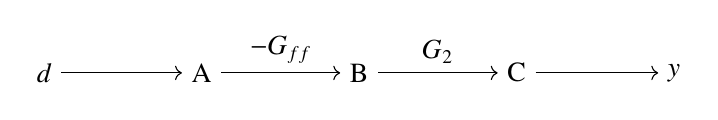
\begin{tikzpicture}[auto,node distance=2cm]
    \node[] (1) {A};
    \node[] (0) [left of =1] {$d$};
    \node[] (2) [right of=1] {B};
    \node[] (3) [right of=2] {C};
    \node[] (5) [right of=3] {$y$};
    \draw [->] (0) -- (1);
    \draw [->] (1) -- (2)node[midway] {$-G_{ff}$};
    \draw [->] (2) -- (3)node[midway] {$G_2$};
    \draw [->] (3) -- (5);
    \end{tikzpicture}    
    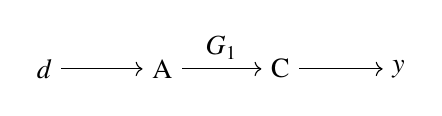
\begin{tikzpicture}[auto,node distance=1.5cm]
    \node[] (1) {A};
    \node[] (0) [left of =1] {$d$};
    \node[] (3) [right of=1] {C};
    \node[] (5) [right of=3] {$y$};
    \draw [->] (0) -- (1);
    \draw [->] (1) -- (3) node[midway] {$G_1$};
    \draw [->] (3) -- (5);
    \end{tikzpicture}   
\end{center} 
For these paths, 
\begin{align}
    &P_1 = -G_2 G_{ff}\\
    &P_2 = G_1 \\
    &\Delta_1  = \Delta_2=1-\brak{0}\\
    &\Delta =  1-\brak{0}=1
\end{align}
From \eqref{Gate22.CH23.eqn: 1} and \tabref{Gate22.CH23.tab: 1}
\begin{align}
    H=G_1-G_2G_{ff}
\end{align}
Since $H=0$, 
\begin{align}
    &G_1-G_2G_{ff} = 0\\
    \implies &G_{ff} = \frac{G_1}{G_2} =\frac{2}{3} \frac{8s+1}{5s+1}
\end{align}
\end{enumerate}
%\end{document}

 
